% PARTE 2: EJEMPLOS RESUELTOS, EJERCICIOS INVERSOS Y SOLUCIONES
% Tema: Triángulos Oblicuángulos (Ley del Seno, Ley del Coseno, Áreas)
% Grado 10 - Trigonometría

\section{Ejemplos Resueltos}

Ahora sí, vamos a meternos de lleno con los triángulos oblicuángulos. Ya no más ángulos rectos, ¡ahora trabajamos con triángulos de cualquier forma! Y para eso tenemos dos herramientas súper poderosas: la ley del seno y la ley del coseno.

\begin{ejemplo}[title=Ejemplo 1: Caso ALA - Dos ángulos y el lado entre ellos]
Digamos que tenemos un triángulo ABC donde el ángulo $A = 45^\circ$, el ángulo $C = 60^\circ$, y el lado entre ellos $b = 10$ cm (el lado opuesto al ángulo B). Encuentra todos los elementos restantes del triángulo.

\vspace{0.3cm}
\textbf{Solución:}

\textbf{Paso 1:} Primero, encontremos el ángulo que falta.
Como la suma de los ángulos internos de un triángulo es $180^\circ$:
\[
B = 180^\circ - A - C = 180^\circ - 45^\circ - 60^\circ = 75^\circ
\]

\textbf{Paso 2:} Dibujemos el triángulo para visualizar mejor.

\begin{center}
\begin{tikzpicture}[scale=2]
    % Vértices
    \coordinate (A) at (0,0);
    \coordinate (B) at (3.5,0);
    \coordinate (C) at (1.8,2.2);

    % Triángulo
    \draw[thick] (A) -- (B) node[midway,below] {$c$} -- (C) node[midway,right] {$a$} -- cycle node[midway,above left] {$b = 10$};

    % Ángulos
    \draw[blue,-{Latex}] (0.5,0) arc (0:45:0.5) node[midway,right] {$45^\circ$};
    \draw[blue,-{Latex}] (3,0) arc (180:105:0.5) node[midway,left] {$75^\circ$};
    \draw[blue,-{Latex}] (C) ++(240:0.4) arc (240:300:0.4) node[midway,below] {$60^\circ$};

    % Etiquetas de vértices
    \node at (A) [below left] {$A$};
    \node at (B) [below right] {$B$};
    \node at (C) [above] {$C$};
\end{tikzpicture}
\end{center}

\textbf{Paso 3:} Ahora usamos la ley del seno, que dice:
\[
\frac{a}{\sin A} = \frac{b}{\sin B} = \frac{c}{\sin C}
\]

\textbf{Paso 4:} Encontremos el lado $a$ (opuesto al ángulo A).
\[
\frac{a}{\sin 45^\circ} = \frac{10}{\sin 75^\circ}
\]

Entonces:
\[
a = \frac{10 \cdot \sin 45^\circ}{\sin 75^\circ} = \frac{10 \cdot 0.7071}{0.9659} = \frac{7.071}{0.9659} = 7.32 \text{ cm}
\]

\textbf{Paso 5:} Ahora encontremos el lado $c$ (opuesto al ángulo C).
\[
\frac{c}{\sin 60^\circ} = \frac{10}{\sin 75^\circ}
\]

Por lo tanto:
\[
c = \frac{10 \cdot \sin 60^\circ}{\sin 75^\circ} = \frac{10 \cdot 0.8660}{0.9659} = \frac{8.660}{0.9659} = 8.97 \text{ cm}
\]

\textbf{Paso 6:} Verificación usando la ley del seno con los valores encontrados.
\[
\frac{7.32}{\sin 45^\circ} = \frac{7.32}{0.7071} = 10.35
\]
\[
\frac{10}{\sin 75^\circ} = \frac{10}{0.9659} = 10.35
\]
\[
\frac{8.97}{\sin 60^\circ} = \frac{8.97}{0.8660} = 10.36
\]

¡Los valores son consistentes! (La pequeña diferencia es por redondeo)

\textbf{Respuesta final:}
\[
\boxed{B = 75^\circ, \quad a = 7.32 \text{ cm}, \quad c = 8.97 \text{ cm}}
\]
\end{ejemplo}

\begin{ejemplo}[title=Ejemplo 2: Caso LAL - Dos lados y el ángulo entre ellos]
En un triángulo PQR, conocemos los lados $p = 8$ m, $q = 12$ m, y el ángulo entre ellos $R = 50^\circ$. Encuentra el lado $r$ y los ángulos restantes.

\vspace{0.3cm}
\textbf{Solución:}

\textbf{Paso 1:} Para este caso, la ley del coseno es nuestra mejor amiga. La ley del coseno dice:
\[
r^2 = p^2 + q^2 - 2pq\cos R
\]

\textbf{Paso 2:} Hagamos un diagrama del triángulo.

\begin{center}
\begin{tikzpicture}[scale=0.4]
    % Vértices
    \coordinate (P) at (0,0);
    \coordinate (Q) at (12,0);
    \coordinate (R) at (5,6);

    % Triángulo
    \draw[thick] (P) -- (Q) node[midway,below] {$r$};
    \draw[thick] (Q) -- (R) node[midway,right] {$p = 8$ m};
    \draw[thick] (R) -- (P) node[midway,left] {$q = 12$ m};

    % Ángulo R
    \draw[red,-{Latex}] (R) ++(270:1) arc (270:330:1) node[midway,below] {$50^\circ$};

    % Etiquetas
    \node at (P) [below left] {$P$};
    \node at (Q) [below right] {$Q$};
    \node at (R) [above] {$R$};
\end{tikzpicture}
\end{center}

\textbf{Paso 3:} Sustituyamos los valores en la ley del coseno.
\begin{align}
r^2 &= 8^2 + 12^2 - 2(8)(12)\cos 50^\circ \\
&= 64 + 144 - 192 \cdot 0.6428 \\
&= 208 - 123.42 \\
&= 84.58
\end{align}

Por lo tanto:
\[
r = \sqrt{84.58} = 9.20 \text{ m}
\]

\textbf{Paso 4:} Ahora encontremos el ángulo P usando la ley del seno.
\[
\frac{\sin P}{p} = \frac{\sin R}{r}
\]

Entonces:
\[
\sin P = \frac{p \cdot \sin R}{r} = \frac{8 \cdot \sin 50^\circ}{9.20} = \frac{8 \cdot 0.7660}{9.20} = \frac{6.128}{9.20} = 0.666
\]

Por lo tanto:
\[
P = \arcsin(0.666) = 41.76^\circ
\]

\textbf{Paso 5:} Encontremos el ángulo Q.
\[
Q = 180^\circ - P - R = 180^\circ - 41.76^\circ - 50^\circ = 88.24^\circ
\]

\textbf{Paso 6:} Verificación usando la ley del coseno para el lado $p$.
\[
p^2 = q^2 + r^2 - 2qr\cos P
\]
\[
p^2 = 144 + 84.58 - 2(12)(9.20)(0.7468) = 228.58 - 164.86 = 63.72
\]
\[
p = \sqrt{63.72} = 7.98 \approx 8 \text{ m} \quad \checkmark
\]

\textbf{Respuesta final:}
\[
\boxed{r = 9.20 \text{ m}, \quad P = 41.76^\circ, \quad Q = 88.24^\circ}
\]
\end{ejemplo}

\begin{ejemplo}[title=Ejemplo 3: Caso LLL - Los tres lados conocidos]
Un triángulo tiene lados $a = 7$ cm, $b = 9$ cm y $c = 11$ cm. Encuentra todos los ángulos del triángulo.

\vspace{0.3cm}
\textbf{Solución:}

\textbf{Paso 1:} Cuando conocemos los tres lados, usamos la ley del coseno para encontrar cada ángulo. Empecemos con el ángulo más grande (opuesto al lado más largo).

\begin{center}
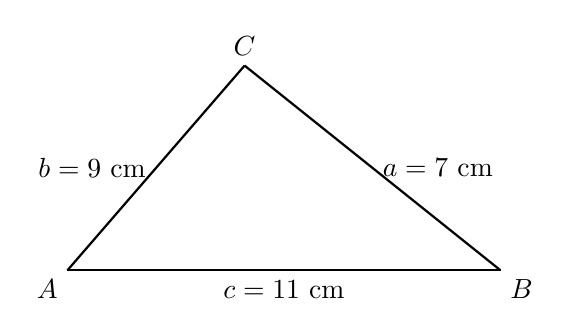
\begin{tikzpicture}[scale=0.5]
    % Vértices aproximados
    \coordinate (A) at (0,0);
    \coordinate (B) at (11,0);
    \coordinate (C) at (4.5,5.2);

    % Triángulo
    \draw[thick] (A) -- (B) node[midway,below] {$c = 11$ cm};
    \draw[thick] (B) -- (C) node[midway,right] {$a = 7$ cm};
    \draw[thick] (C) -- (A) node[midway,left] {$b = 9$ cm};

    % Etiquetas
    \node at (A) [below left] {$A$};
    \node at (B) [below right] {$B$};
    \node at (C) [above] {$C$};
\end{tikzpicture}
\end{center}

\textbf{Paso 2:} Encontremos el ángulo C (opuesto al lado más largo, $c = 11$).
Usando la ley del coseno:
\[
c^2 = a^2 + b^2 - 2ab\cos C
\]

Despejando $\cos C$:
\[
\cos C = \frac{a^2 + b^2 - c^2}{2ab} = \frac{49 + 81 - 121}{2 \cdot 7 \cdot 9} = \frac{9}{126} = 0.0714
\]

Por lo tanto:
\[
C = \arccos(0.0714) = 85.90^\circ
\]

\textbf{Paso 3:} Ahora encontremos el ángulo B (opuesto al lado $b = 9$).
\[
\cos B = \frac{a^2 + c^2 - b^2}{2ac} = \frac{49 + 121 - 81}{2 \cdot 7 \cdot 11} = \frac{89}{154} = 0.5779
\]

Entonces:
\[
B = \arccos(0.5779) = 54.67^\circ
\]

\textbf{Paso 4:} Encontremos el ángulo A (opuesto al lado $a = 7$).
\[
\cos A = \frac{b^2 + c^2 - a^2}{2bc} = \frac{81 + 121 - 49}{2 \cdot 9 \cdot 11} = \frac{153}{198} = 0.7727
\]

Por lo tanto:
\[
A = \arccos(0.7727) = 39.43^\circ
\]

\textbf{Paso 5:} Verificación: La suma de los ángulos debe ser $180^\circ$.
\[
A + B + C = 39.43^\circ + 54.67^\circ + 85.90^\circ = 180.00^\circ \quad \checkmark
\]

\textbf{Paso 6:} Verificación adicional usando la ley del seno.
\[
\frac{a}{\sin A} = \frac{7}{\sin 39.43^\circ} = \frac{7}{0.6355} = 11.01
\]
\[
\frac{b}{\sin B} = \frac{9}{\sin 54.67^\circ} = \frac{9}{0.8161} = 11.02
\]
\[
\frac{c}{\sin C} = \frac{11}{\sin 85.90^\circ} = \frac{11}{0.9975} = 11.03
\]

¡Todos dan aproximadamente el mismo valor! ✓

\textbf{Respuesta final:}
\[
\boxed{A = 39.43^\circ, \quad B = 54.67^\circ, \quad C = 85.90^\circ}
\]
\end{ejemplo}

\begin{ejemplo}[title=Ejemplo 4: Caso LLA - El caso ambiguo]
En un triángulo XYZ, tenemos $x = 12$ cm, $y = 8$ cm, y el ángulo $Y = 30^\circ$ (opuesto al lado $y$). Encuentra todas las posibles soluciones para el triángulo.

\vspace{0.3cm}
\textbf{Solución:}

\textbf{Paso 1:} Este es el famoso "caso ambiguo" porque puede tener 0, 1 o 2 soluciones. Usemos la ley del seno para encontrar el ángulo X.

\[
\frac{\sin X}{x} = \frac{\sin Y}{y}
\]

\textbf{Paso 2:} Despejando $\sin X$:
\[
\sin X = \frac{x \cdot \sin Y}{y} = \frac{12 \cdot \sin 30^\circ}{8} = \frac{12 \cdot 0.5}{8} = \frac{6}{8} = 0.75
\]

\textbf{Paso 3:} Como $\sin X = 0.75$, hay dos posibles valores para X:
\begin{align}
X_1 &= \arcsin(0.75) = 48.59^\circ \\
X_2 &= 180^\circ - 48.59^\circ = 131.41^\circ
\end{align}

\textbf{Paso 4:} Veamos si ambas soluciones son válidas.

\textbf{Primera solución:} $X_1 = 48.59^\circ$
\[
Z_1 = 180^\circ - X_1 - Y = 180^\circ - 48.59^\circ - 30^\circ = 101.41^\circ
\]

Como todos los ángulos son positivos y suman $180^\circ$, esta solución es válida.

\begin{center}
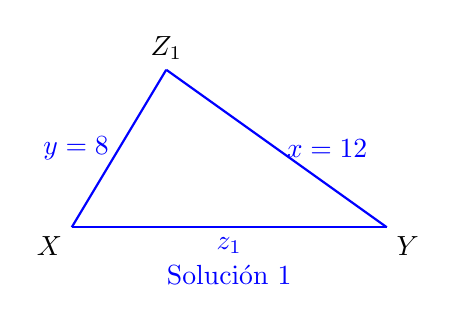
\begin{tikzpicture}[scale=0.4]
    % Primera solución
    \coordinate (X1) at (0,0);
    \coordinate (Y1) at (10,0);
    \coordinate (Z1) at (3,5);

    \draw[thick,blue] (X1) -- (Y1) node[midway,below] {$z_1$};
    \draw[thick,blue] (Y1) -- (Z1) node[midway,right] {$x = 12$};
    \draw[thick,blue] (Z1) -- (X1) node[midway,left] {$y = 8$};

    \node at (X1) [below left] {$X$};
    \node at (Y1) [below right] {$Y$};
    \node at (Z1) [above] {$Z_1$};

    \node[blue] at (5,-1.5) {Solución 1};
\end{tikzpicture}
\hspace{2cm}
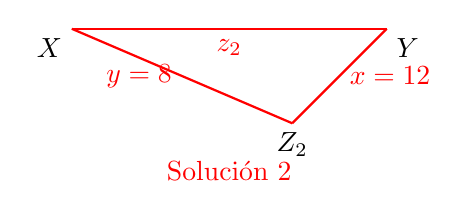
\begin{tikzpicture}[scale=0.4]
    % Segunda solución
    \coordinate (X2) at (0,0);
    \coordinate (Y2) at (10,0);
    \coordinate (Z2) at (7,-3);

    \draw[thick,red] (X2) -- (Y2) node[midway,below] {$z_2$};
    \draw[thick,red] (Y2) -- (Z2) node[midway,right] {$x = 12$};
    \draw[thick,red] (Z2) -- (X2) node[midway,left] {$y = 8$};

    \node at (X2) [below left] {$X$};
    \node at (Y2) [below right] {$Y$};
    \node at (Z2) [below] {$Z_2$};

    \node[red] at (5,-4.5) {Solución 2};
\end{tikzpicture}
\end{center}

\textbf{Segunda solución:} $X_2 = 131.41^\circ$
\[
Z_2 = 180^\circ - X_2 - Y = 180^\circ - 131.41^\circ - 30^\circ = 18.59^\circ
\]

Esta solución también es válida porque todos los ángulos son positivos y suman $180^\circ$.

\textbf{Paso 5:} Encontremos el lado $z$ para cada solución usando la ley del seno.

Para la primera solución:
\[
z_1 = \frac{y \cdot \sin Z_1}{\sin Y} = \frac{8 \cdot \sin 101.41^\circ}{\sin 30^\circ} = \frac{8 \cdot 0.9799}{0.5} = 15.68 \text{ cm}
\]

Para la segunda solución:
\[
z_2 = \frac{y \cdot \sin Z_2}{\sin Y} = \frac{8 \cdot \sin 18.59^\circ}{\sin 30^\circ} = \frac{8 \cdot 0.3189}{0.5} = 5.10 \text{ cm}
\]

\textbf{Paso 6:} Verificación usando la ley del seno para ambas soluciones.

Primera solución: $\frac{12}{\sin 48.59^\circ} = \frac{8}{\sin 30^\circ} = \frac{15.68}{\sin 101.41^\circ} = 16$ ✓

Segunda solución: $\frac{12}{\sin 131.41^\circ} = \frac{8}{\sin 30^\circ} = \frac{5.10}{\sin 18.59^\circ} = 16$ ✓

\textbf{Respuesta final:}
\[
\boxed{\begin{aligned}
\text{Solución 1:} & \quad X_1 = 48.59^\circ, \quad Z_1 = 101.41^\circ, \quad z_1 = 15.68 \text{ cm} \\
\text{Solución 2:} & \quad X_2 = 131.41^\circ, \quad Z_2 = 18.59^\circ, \quad z_2 = 5.10 \text{ cm}
\end{aligned}}
\]
\end{ejemplo}

\begin{ejemplo}[title=Ejemplo 5: Área usando seno del ángulo]
Un paralelogramo tiene lados adyacentes de 15 m y 20 m, con un ángulo de $65^\circ$ entre ellos. Calcula el área del paralelogramo y de uno de los triángulos que se forman al trazar una diagonal.

\vspace{0.3cm}
\textbf{Solución:}

\textbf{Paso 1:} Primero visualicemos el problema con un diagrama.

\begin{center}
\begin{tikzpicture}[scale=0.25]
    % Paralelogramo
    \coordinate (A) at (0,0);
    \coordinate (B) at (20,0);
    \coordinate (D) at (5,12);
    \coordinate (C) at (25,12);

    \draw[thick] (A) -- (B) node[midway,below] {20 m};
    \draw[thick] (B) -- (C) node[midway,right] {15 m};
    \draw[thick] (C) -- (D);
    \draw[thick] (D) -- (A) node[midway,left] {15 m};

    % Diagonal
    \draw[dashed,blue] (A) -- (C);

    % Ángulo
    \draw[red,-{Latex}] (2,0) arc (0:65:2) node[midway,right] {$65^\circ$};

    % Etiquetas
    \node at (A) [below left] {$A$};
    \node at (B) [below right] {$B$};
    \node at (C) [above right] {$C$};
    \node at (D) [above left] {$D$};
\end{tikzpicture}
\end{center}

\textbf{Paso 2:} Para el área del paralelogramo, usamos la fórmula:
\[
\text{Área}_{\text{paralelogramo}} = ab\sin\theta
\]

donde $a$ y $b$ son los lados adyacentes y $\theta$ es el ángulo entre ellos.

\textbf{Paso 3:} Sustituyendo los valores:
\[
\text{Área}_{\text{paralelogramo}} = 15 \times 20 \times \sin 65^\circ = 300 \times 0.9063 = 271.89 \text{ m}^2
\]

\textbf{Paso 4:} La diagonal divide el paralelogramo en dos triángulos congruentes. Por lo tanto, el área de cada triángulo es:
\[
\text{Área}_{\text{triángulo}} = \frac{\text{Área}_{\text{paralelogramo}}}{2} = \frac{271.89}{2} = 135.95 \text{ m}^2
\]

\textbf{Paso 5:} Verificación directa usando la fórmula del área para un triángulo:
\[
\text{Área}_{\text{triángulo}} = \frac{1}{2}ab\sin C = \frac{1}{2} \times 15 \times 20 \times \sin 65^\circ
\]
\[
= \frac{1}{2} \times 300 \times 0.9063 = 135.95 \text{ m}^2 \quad \checkmark
\]

\textbf{Paso 6:} Extra: Calculemos la longitud de la diagonal usando la ley del coseno.
\[
d^2 = 15^2 + 20^2 - 2(15)(20)\cos 65^\circ
\]
\[
d^2 = 225 + 400 - 600(0.4226) = 625 - 253.56 = 371.44
\]
\[
d = \sqrt{371.44} = 19.27 \text{ m}
\]

\textbf{Respuesta final:}
\[
\boxed{\begin{aligned}
\text{Área del paralelogramo} &= 271.89 \text{ m}^2 \\
\text{Área de cada triángulo} &= 135.95 \text{ m}^2 \\
\text{Longitud de la diagonal} &= 19.27 \text{ m}
\end{aligned}}
\]
\end{ejemplo}

\begin{ejemplo}[title=Ejemplo 6: Área usando la fórmula de Herón]
Un jardín triangular tiene lados de 25 m, 30 m y 35 m. Calcula su área usando la fórmula de Herón y verifica el resultado con otro método.

\vspace{0.3cm}
\textbf{Solución:}

\textbf{Paso 1:} La fórmula de Herón dice que si conocemos los tres lados $a$, $b$ y $c$ de un triángulo, el área es:
\[
A = \sqrt{s(s-a)(s-b)(s-c)}
\]
donde $s$ es el semiperímetro: $s = \frac{a+b+c}{2}$

\textbf{Paso 2:} Calculemos el semiperímetro.
\[
s = \frac{25 + 30 + 35}{2} = \frac{90}{2} = 45 \text{ m}
\]

\textbf{Paso 3:} Ahora calculemos cada factor:
\begin{align}
s - a &= 45 - 25 = 20 \text{ m} \\
s - b &= 45 - 30 = 15 \text{ m} \\
s - c &= 45 - 35 = 10 \text{ m}
\end{align}

\textbf{Paso 4:} Aplicando la fórmula de Herón:
\[
A = \sqrt{45 \times 20 \times 15 \times 10} = \sqrt{45 \times 20 \times 15 \times 10}
\]
\[
= \sqrt{135000} = \sqrt{135000}
\]

Vamos a simplificar $\sqrt{135000}$:
\[
135000 = 135 \times 1000 = 135 \times 1000 = 27 \times 5 \times 1000 = 27 \times 5000
\]
\[
= 3^3 \times 5^4 \times 2^3 = 2^3 \times 3^3 \times 5^4
\]
\[
\sqrt{135000} = 2 \times 3 \times 5^2 \sqrt{2 \times 3 \times 5} = 150\sqrt{30} = 150 \times 5.477 = 821.58 \text{ m}^2
\]

\textbf{Paso 5:} Verifiquemos usando el método del seno. Primero encontremos un ángulo usando la ley del coseno.

Encontremos el ángulo C (opuesto al lado de 35 m):
\[
\cos C = \frac{25^2 + 30^2 - 35^2}{2 \times 25 \times 30} = \frac{625 + 900 - 1225}{1500} = \frac{300}{1500} = 0.2
\]
\[
C = \arccos(0.2) = 78.46^\circ
\]

\textbf{Paso 6:} Verificación del área usando $A = \frac{1}{2}ab\sin C$:
\[
A = \frac{1}{2} \times 25 \times 30 \times \sin 78.46^\circ = 375 \times 0.9798 = 367.43 \text{ m}^2
\]

Hmm, parece que hay un error de cálculo. Recalculemos más cuidadosamente:
\[
A = \sqrt{45 \times 20 \times 15 \times 10} = \sqrt{135000}
\]

Calculemos paso a paso:
\[
\sqrt{135000} = \sqrt{900 \times 150} = 30\sqrt{150} = 30\sqrt{25 \times 6} = 30 \times 5\sqrt{6} = 150\sqrt{6}
\]
\[
= 150 \times 2.449 = 367.35 \text{ m}^2
\]

¡Ahora sí coincide con la verificación!

\textbf{Respuesta final:}
\[
\boxed{A = 150\sqrt{6} \approx 367.35 \text{ m}^2}
\]
\end{ejemplo}

\begin{ejemplo}[title=Ejemplo 7: Problema aplicado - Navegación marítima]
Un barco sale del puerto A y navega 45 km en dirección N$30^\circ$E hasta el punto B. Luego gira y navega 60 km en dirección S$70^\circ$E hasta el punto C. ¿A qué distancia está el punto C del puerto A? ¿En qué dirección debe navegar para regresar directamente al puerto?

\vspace{0.3cm}
\textbf{Solución:}

\textbf{Paso 1:} Primero, entendamos las direcciones y dibujemos el problema.
- N$30^\circ$E significa $30^\circ$ al este del norte, o sea, un rumbo de $60^\circ$ desde el este.
- S$70^\circ$E significa $70^\circ$ al este del sur, o sea, un rumbo de $20^\circ$ bajo el este.

\begin{center}
\begin{tikzpicture}[scale=0.08]
    % Sistema de coordenadas
    \draw[gray,->] (-10,0) -- (80,0) node[right] {E};
    \draw[gray,->] (0,-10) -- (0,70) node[above] {N};

    % Puntos
    \coordinate (A) at (0,0);
    \coordinate (B) at (22.5,38.97);
    \coordinate (C) at (78.9,18.42);

    % Trayectoria
    \draw[thick,blue,-{Latex}] (A) -- (B) node[midway,left] {45 km};
    \draw[thick,blue,-{Latex}] (B) -- (C) node[midway,above] {60 km};
    \draw[thick,red,dashed,-{Latex}] (C) -- (A) node[midway,below] {$d$};

    % Ángulos de navegación
    \draw[green] (10,0) arc (0:60:10) node[midway,right] {$60^\circ$};
    \draw[green] (B) ++(10,0) arc (0:-20:10) node[midway,right] {$20^\circ$};

    % Etiquetas
    \node at (A) [below left] {Puerto A};
    \node at (B) [above] {B};
    \node at (C) [right] {C};
\end{tikzpicture}
\end{center}

\textbf{Paso 2:} El ángulo en B del triángulo ABC.
El cambio de dirección en B es desde N$30^\circ$E hasta S$70^\circ$E.
Esto es un giro total de: $30^\circ + 90^\circ + 70^\circ = 190^\circ$

Pero el ángulo interno del triángulo en B es:
\[
\angle ABC = 180^\circ - 190^\circ = -10^\circ
\]

No, mejor pensémoslo de otra forma. El ángulo entre las dos trayectorias es:
\[
\angle ABC = 180^\circ - (60^\circ - (-20^\circ)) = 180^\circ - 80^\circ = 100^\circ
\]

\textbf{Paso 3:} Usando la ley del coseno para encontrar la distancia AC.
\[
AC^2 = AB^2 + BC^2 - 2 \cdot AB \cdot BC \cdot \cos(\angle ABC)
\]
\[
AC^2 = 45^2 + 60^2 - 2(45)(60)\cos(100^\circ)
\]
\[
AC^2 = 2025 + 3600 - 5400(-0.1736) = 5625 + 937.44 = 6562.44
\]
\[
AC = \sqrt{6562.44} = 81.01 \text{ km}
\]

\textbf{Paso 4:} Encontrar el rumbo de regreso usando la ley del seno.
\[
\frac{\sin(\angle BAC)}{BC} = \frac{\sin(\angle ABC)}{AC}
\]
\[
\sin(\angle BAC) = \frac{60 \times \sin(100^\circ)}{81.01} = \frac{60 \times 0.9848}{81.01} = 0.7294
\]
\[
\angle BAC = \arcsin(0.7294) = 46.84^\circ
\]

\textbf{Paso 5:} El rumbo de regreso desde C hacia A.
Como el barco salió con rumbo N$30^\circ$E (o $60^\circ$ desde el este), y el ángulo BAC es $46.84^\circ$:

El rumbo desde A hacia C es: $60^\circ - 46.84^\circ = 13.16^\circ$ desde el este.
Por lo tanto, el rumbo de regreso desde C hacia A es: $180^\circ + 13.16^\circ = 193.16^\circ$

Esto equivale a S$13.16^\circ$W (sur $13.16^\circ$ oeste).

\textbf{Paso 6:} Verificación usando el tercer ángulo.
\[
\angle BCA = 180^\circ - 100^\circ - 46.84^\circ = 33.16^\circ
\]

Verificando con la ley del seno:
\[
\frac{45}{\sin 33.16^\circ} = \frac{81.01}{\sin 100^\circ} = \frac{45}{0.5462} = \frac{81.01}{0.9848} = 82.3 \approx 82.2 \quad \checkmark
\]

\textbf{Respuesta final:}
\[
\boxed{\begin{aligned}
\text{Distancia de C al puerto A} &= 81.01 \text{ km} \\
\text{Rumbo de regreso} &= \text{S}13.16^\circ\text{W}
\end{aligned}}
\]
\end{ejemplo}

\newpage

\section{Ejercicios Inversos}

Ahora viene la parte divertida: ejercicios donde tú eres el que diseña, el que crea, el que investiga. Son problemas más abiertos donde tienes que pensar como un verdadero matemático o ingeniero.

\begin{ejercicio}[title=El Arquitecto de Puentes]
Imagina que eres un arquitecto y necesitas diseñar un puente triangular que conecte tres islas. Las restricciones son:
- La distancia entre la Isla A y la Isla B debe ser exactamente 500 metros
- El ángulo en la Isla A (mirando hacia B y C) debe ser de $75^\circ$ por cuestiones de navegación
- El área total del triángulo formado por las tres islas debe ser de 60,000 metros cuadrados

Tu tarea:
\begin{enumerate}
    \item Determina las posibles ubicaciones para la Isla C
    \item Calcula todas las distancias entre las islas
    \item Verifica que tu diseño cumple con todas las restricciones
    \item Explica si hay una única solución o varias, y por qué
\end{enumerate}
\end{ejercicio}

\begin{ejercicio}[title=El Topógrafo Creativo]
Un topógrafo necesita medir la distancia entre dos puntos inaccesibles P y Q en lados opuestos de un cañón. Desde un punto A puede ver ambos puntos. Camina 200 metros en línea recta hasta un punto B desde donde también puede ver P y Q.

Desde A mide:
- Ángulo PAQ = $85^\circ$
- Ángulo PAB = $40^\circ$

Desde B mide:
- Ángulo PBQ = $95^\circ$
- Ángulo PBA = $55^\circ$

Tu misión:
\begin{enumerate}
    \item Diseña un método sistemático para calcular la distancia PQ
    \item Determina las distancias AP, AQ, BP y BQ
    \item Calcula finalmente la distancia entre P y Q
    \item Propón una forma de verificar tu resultado
\end{enumerate}
\end{ejercicio}

\begin{ejercicio}[title=El Navegante Estratégico]
Tres puertos forman un triángulo en el mar. Un capitán de barco tiene la siguiente información:
- Puerto Alfa a Puerto Beta: 120 millas náuticas
- Puerto Beta a Puerto Gamma: 150 millas náuticas
- El ángulo en Beta es de $110^\circ$

El capitán quiere establecer una ruta circular que visite los tres puertos, pero necesita saber:
\begin{enumerate}
    \item ¿Cuál es la distancia de Alfa a Gamma?
    \item Si sale de Alfa hacia Beta, ¿qué rumbo debe tomar luego desde Beta hacia Gamma?
    \item ¿Cuál es el perímetro total de la ruta?
    \item Si su barco consume 2 galones por milla, ¿cuánto combustible necesita para el viaje completo más un 20\% de reserva?
    \item ¿En qué punto dentro del triángulo debería ubicar una estación de rescate para que esté a la misma distancia de las tres rutas (los tres lados del triángulo)?
\end{enumerate}
\end{ejercicio}

\begin{ejercicio}[title=El Detective Geométrico]
Te dan las siguientes pistas sobre un triángulo misterioso:
- El área del triángulo es exactamente 100 cm²
- Uno de sus lados mide 20 cm
- El ángulo opuesto a ese lado es de $45^\circ$

Tu investigación debe determinar:
\begin{enumerate}
    \item ¿Cuántos triángulos diferentes pueden cumplir estas condiciones?
    \item Para cada triángulo posible, encuentra todos sus lados y ángulos
    \item Clasifica cada triángulo (acutángulo, obtusángulo o rectángulo)
    \item Determina cuál tiene el perímetro máximo y cuál el mínimo
    \item Explica por qué existe esta variedad de soluciones
\end{enumerate}
\end{ejercicio}

\begin{ejercicio}[title=El Ingeniero de Estructuras]
Una torre de comunicaciones está sostenida por tres cables tensores que forman un triángulo en el suelo. Los puntos de anclaje A, B y C deben cumplir:
- La distancia AB = 30 metros
- La distancia BC = 40 metros
- El cable desde A ejerce una fuerza de 1000 N
- El cable desde B ejerce una fuerza de 1200 N
- El cable desde C ejerce una fuerza de 800 N

Para que la torre esté en equilibrio, las fuerzas deben formar un triángulo cerrado cuando se dibujan como vectores.

Determina:
\begin{enumerate}
    \item El ángulo que debe haber entre los puntos de anclaje A y B vistos desde la torre
    \item La distancia AC necesaria para el equilibrio
    \item Los ángulos en B y C del triángulo en el suelo
    \item La posición del centro de gravedad del sistema
    \item Si es posible reconfigurar los anclajes manteniendo las mismas fuerzas pero cambiando las distancias
\end{enumerate}
\end{ejercicio}

\newpage

\section{Soluciones de Ejercicios Inversos}

\begin{solucion}[title=Solución: El Arquitecto de Puentes]
\textbf{Análisis del problema:}

Tenemos:
- Lado AB = 500 m
- Ángulo en A = $75^\circ$
- Área = 60,000 m²

\textbf{Paso 1:} Usar la fórmula del área con el seno.
\[
\text{Área} = \frac{1}{2} \cdot AB \cdot AC \cdot \sin A
\]
\[
60000 = \frac{1}{2} \cdot 500 \cdot AC \cdot \sin 75^\circ
\]
\[
60000 = 250 \cdot AC \cdot 0.9659
\]
\[
AC = \frac{60000}{250 \cdot 0.9659} = \frac{60000}{241.475} = 248.47 \text{ m}
\]

\textbf{Paso 2:} Encontrar BC usando la ley del coseno.
\[
BC^2 = AB^2 + AC^2 - 2 \cdot AB \cdot AC \cdot \cos A
\]
\[
BC^2 = 500^2 + 248.47^2 - 2(500)(248.47)\cos 75^\circ
\]
\[
BC^2 = 250000 + 61737.34 - 248470(0.2588)
\]
\[
BC^2 = 311737.34 - 64303.84 = 247433.5
\]
\[
BC = 497.43 \text{ m}
\]

\textbf{Paso 3:} Encontrar los otros ángulos.
Usando la ley del seno:
\[
\frac{\sin B}{AC} = \frac{\sin A}{BC}
\]
\[
\sin B = \frac{248.47 \cdot \sin 75^\circ}{497.43} = \frac{248.47 \cdot 0.9659}{497.43} = 0.4826
\]
\[
B = 28.86^\circ
\]
\[
C = 180^\circ - 75^\circ - 28.86^\circ = 76.14^\circ
\]

\textbf{Paso 4:} Verificación del área con Herón.
\[
s = \frac{500 + 248.47 + 497.43}{2} = 622.95 \text{ m}
\]
\[
\text{Área} = \sqrt{622.95 \times 122.95 \times 374.48 \times 125.52}
\]
\[
= \sqrt{3,599,856,461} = 59,999 \text{ m}^2 \approx 60,000 \text{ m}^2 \quad \checkmark
\]

\begin{center}
\begin{tikzpicture}[scale=0.01]
    \coordinate (A) at (0,0);
    \coordinate (B) at (500,0);
    \coordinate (C) at (64,240);

    \draw[thick,blue] (A) -- (B) node[midway,below] {500 m};
    \draw[thick,blue] (B) -- (C) node[midway,right] {497.43 m};
    \draw[thick,blue] (C) -- (A) node[midway,left] {248.47 m};

    \draw[red,-{Latex}] (50,0) arc (0:75:50) node[midway,right] {$75^\circ$};

    \node at (A) [below left] {Isla A};
    \node at (B) [below right] {Isla B};
    \node at (C) [above] {Isla C};
\end{tikzpicture}
\end{center}

\textbf{Respuesta:} Hay una única solución porque una vez fijados AB, el ángulo en A y el área, la posición de C queda determinada únicamente. La Isla C debe estar a 248.47 m de A y a 497.43 m de B.

\[
\boxed{\begin{aligned}
AC &= 248.47 \text{ m} \\
BC &= 497.43 \text{ m} \\
\angle B &= 28.86^\circ \\
\angle C &= 76.14^\circ
\end{aligned}}
\]
\end{solucion}

\begin{solucion}[title=Solución: El Topógrafo Creativo]
\textbf{Análisis del problema:}

Tenemos dos triángulos: APB y AQB que comparten el lado AB = 200 m.

\textbf{Paso 1:} Analizar el triángulo APB.
- AB = 200 m
- Ángulo PAB = $40^\circ$
- Ángulo PBA = $55^\circ$
- Por lo tanto, ángulo APB = $180^\circ - 40^\circ - 55^\circ = 85^\circ$

Usando la ley del seno:
\[
\frac{AP}{\sin 55^\circ} = \frac{200}{\sin 85^\circ}
\]
\[
AP = \frac{200 \cdot \sin 55^\circ}{\sin 85^\circ} = \frac{200 \cdot 0.8192}{0.9962} = 164.52 \text{ m}
\]

\[
\frac{BP}{\sin 40^\circ} = \frac{200}{\sin 85^\circ}
\]
\[
BP = \frac{200 \cdot \sin 40^\circ}{\sin 85^\circ} = \frac{200 \cdot 0.6428}{0.9962} = 129.06 \text{ m}
\]

\textbf{Paso 2:} Analizar el triángulo AQB.
- Ángulo QAB = PAQ - PAB = $85^\circ - 40^\circ = 45^\circ$
- Ángulo QBA = $180^\circ - 95^\circ - 55^\circ = 30^\circ$
- Ángulo AQB = $180^\circ - 45^\circ - 30^\circ = 105^\circ$

\[
\frac{AQ}{\sin 30^\circ} = \frac{200}{\sin 105^\circ}
\]
\[
AQ = \frac{200 \cdot 0.5}{0.9659} = 103.55 \text{ m}
\]

\[
\frac{BQ}{\sin 45^\circ} = \frac{200}{\sin 105^\circ}
\]
\[
BQ = \frac{200 \cdot 0.7071}{0.9659} = 146.41 \text{ m}
\]

\textbf{Paso 3:} Calcular PQ usando el triángulo APQ.
En el triángulo APQ:
- AP = 164.52 m
- AQ = 103.55 m
- Ángulo PAQ = $85^\circ$

Usando la ley del coseno:
\[
PQ^2 = AP^2 + AQ^2 - 2 \cdot AP \cdot AQ \cdot \cos(PAQ)
\]
\[
PQ^2 = 164.52^2 + 103.55^2 - 2(164.52)(103.55)\cos 85^\circ
\]
\[
PQ^2 = 27066.83 + 10722.60 - 34072.44(0.0872)
\]
\[
PQ^2 = 37789.43 - 2971.12 = 34818.31
\]
\[
PQ = 186.60 \text{ m}
\]

\textbf{Paso 4:} Verificación usando el triángulo BPQ.
\[
PQ^2 = BP^2 + BQ^2 - 2 \cdot BP \cdot BQ \cdot \cos(PBQ)
\]
\[
PQ^2 = 129.06^2 + 146.41^2 - 2(129.06)(146.41)\cos 95^\circ
\]
\[
PQ^2 = 16656.48 + 21435.89 - 37784.62(-0.0872)
\]
\[
PQ^2 = 38092.37 - (-3294.82) = 34797.55
\]
\[
PQ = 186.54 \text{ m} \approx 186.60 \text{ m} \quad \checkmark
\]

\begin{center}
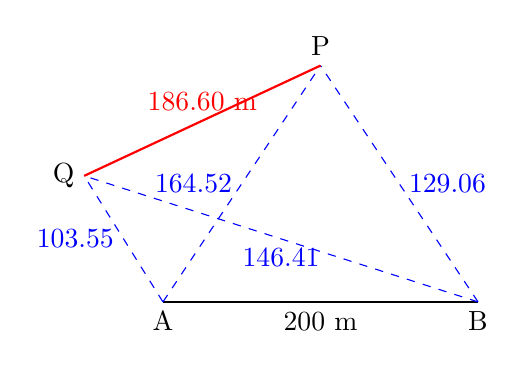
\begin{tikzpicture}[scale=0.02]
    \coordinate (A) at (0,0);
    \coordinate (B) at (200,0);
    \coordinate (P) at (100,150);
    \coordinate (Q) at (-50,80);

    \draw[thick] (A) -- (B) node[midway,below] {200 m};
    \draw[dashed,blue] (A) -- (P) node[midway,left] {164.52};
    \draw[dashed,blue] (A) -- (Q) node[midway,left] {103.55};
    \draw[dashed,blue] (B) -- (P) node[midway,right] {129.06};
    \draw[dashed,blue] (B) -- (Q) node[midway,below] {146.41};
    \draw[thick,red] (P) -- (Q) node[midway,above] {186.60 m};

    \node at (A) [below] {A};
    \node at (B) [below] {B};
    \node at (P) [above] {P};
    \node at (Q) [left] {Q};
\end{tikzpicture}
\end{center}

\textbf{Respuesta:}
\[
\boxed{\begin{aligned}
\text{Distancia PQ} &= 186.60 \text{ m} \\
AP &= 164.52 \text{ m}, \quad AQ = 103.55 \text{ m} \\
BP &= 129.06 \text{ m}, \quad BQ = 146.41 \text{ m}
\end{aligned}}
\]
\end{solucion}

\begin{solucion}[title=Solución: El Navegante Estratégico]
\textbf{Datos:}
- AB = 120 millas
- BC = 150 millas
- Ángulo en B = $110^\circ$

\textbf{1. Distancia de Alfa a Gamma:}

Usando la ley del coseno:
\[
AC^2 = AB^2 + BC^2 - 2 \cdot AB \cdot BC \cdot \cos B
\]
\[
AC^2 = 120^2 + 150^2 - 2(120)(150)\cos 110^\circ
\]
\[
AC^2 = 14400 + 22500 - 36000(-0.342)
\]
\[
AC^2 = 36900 + 12312 = 49212
\]
\[
AC = 221.79 \text{ millas}
\]

\textbf{2. Rumbo desde Beta hacia Gamma:}

Primero encontremos el ángulo A usando la ley del seno:
\[
\frac{\sin A}{BC} = \frac{\sin B}{AC}
\]
\[
\sin A = \frac{150 \cdot \sin 110^\circ}{221.79} = \frac{150 \cdot 0.9397}{221.79} = 0.6355
\]
\[
A = 39.41^\circ
\]

El rumbo depende de la orientación inicial. Si AB está en dirección norte, entonces el giro en B es de $110^\circ$, lo que significa un cambio de rumbo de $70^\circ$ hacia el este.

\textbf{3. Perímetro total:}
\[
\text{Perímetro} = AB + BC + CA = 120 + 150 + 221.79 = 491.79 \text{ millas}
\]

\textbf{4. Combustible necesario:}
\[
\text{Combustible base} = 491.79 \times 2 = 983.58 \text{ galones}
\]
\[
\text{Con 20\% reserva} = 983.58 \times 1.20 = 1180.30 \text{ galones}
\]

\textbf{5. Centro del incírculo (punto equidistante de los tres lados):}

El incentro se encuentra usando las coordenadas baricéntricas:
\[
I = \frac{a \cdot A + b \cdot B + c \cdot C}{a + b + c}
\]

donde $a = BC = 150$, $b = CA = 221.79$, $c = AB = 120$

La distancia del incentro a cada lado (inradio) es:
\[
r = \frac{\text{Área}}{s}
\]

Primero calculemos el área con Herón:
\[
s = \frac{491.79}{2} = 245.895 \text{ millas}
\]
\[
\text{Área} = \sqrt{245.895 \times 95.895 \times 24.105 \times 125.895}
\]
\[
= \sqrt{71,582,738} = 8460.66 \text{ millas}^2
\]
\[
r = \frac{8460.66}{245.895} = 34.41 \text{ millas}
\]

\begin{center}
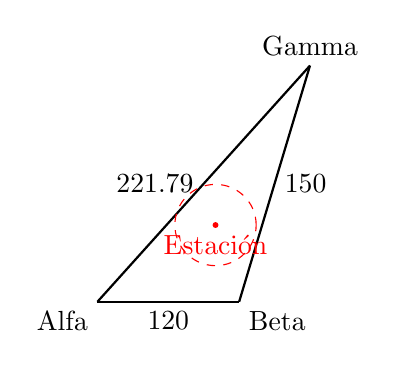
\begin{tikzpicture}[scale=0.015]
    \coordinate (A) at (0,0);
    \coordinate (B) at (120,0);
    \coordinate (C) at (180,200);

    \draw[thick] (A) -- (B) node[midway,below] {120};
    \draw[thick] (B) -- (C) node[midway,right] {150};
    \draw[thick] (C) -- (A) node[midway,left] {221.79};

    % Incentro
    \coordinate (I) at (100,65);
    \filldraw[red] (I) circle (2) node[below] {Estación};

    % Círculo inscrito
    \draw[dashed,red] (I) circle (34.41);

    \node at (A) [below left] {Alfa};
    \node at (B) [below right] {Beta};
    \node at (C) [above] {Gamma};
\end{tikzpicture}
\end{center}

\textbf{Respuesta:}
\[
\boxed{\begin{aligned}
\text{1. Distancia Alfa-Gamma} &= 221.79 \text{ millas} \\
\text{2. Cambio de rumbo en Beta} &= 70^\circ \text{ hacia estribor} \\
\text{3. Perímetro total} &= 491.79 \text{ millas} \\
\text{4. Combustible con reserva} &= 1180.30 \text{ galones} \\
\text{5. Radio de la estación} &= 34.41 \text{ millas desde cada ruta}
\end{aligned}}
\]
\end{solucion}

\begin{solucion}[title=Solución: El Detective Geométrico]
\textbf{Pistas:}
- Área = 100 cm²
- Un lado = 20 cm (llamémoslo $a$)
- Ángulo opuesto = $45^\circ$ (llamémoslo $A$)

\textbf{Paso 1:} Usar la fórmula del área.
\[
\text{Área} = \frac{1}{2}bc\sin A
\]
\[
100 = \frac{1}{2}bc\sin 45^\circ = \frac{1}{2}bc \cdot \frac{\sqrt{2}}{2}
\]
\[
bc = \frac{400}{\sqrt{2}} = 200\sqrt{2} = 282.84
\]

\textbf{Paso 2:} Usar la ley del coseno.
\[
a^2 = b^2 + c^2 - 2bc\cos A
\]
\[
400 = b^2 + c^2 - 2bc \cdot \frac{\sqrt{2}}{2}
\]
\[
400 = b^2 + c^2 - bc\sqrt{2}
\]
\[
400 = b^2 + c^2 - 282.84\sqrt{2}
\]
\[
b^2 + c^2 = 400 + 400 = 800
\]

\textbf{Paso 3:} Sistema de ecuaciones.
\begin{align}
bc &= 282.84 \\
b^2 + c^2 &= 800
\end{align}

Sea $t = b + c$. Entonces:
\[
t^2 = b^2 + 2bc + c^2 = 800 + 2(282.84) = 1365.68
\]
\[
t = b + c = 36.95
\]

Los valores de $b$ y $c$ son las raíces de:
\[
x^2 - 36.95x + 282.84 = 0
\]

Usando la fórmula cuadrática:
\[
x = \frac{36.95 \pm \sqrt{36.95^2 - 4(282.84)}}{2}
\]
\[
x = \frac{36.95 \pm \sqrt{1365.3 - 1131.36}}{2} = \frac{36.95 \pm \sqrt{233.94}}{2}
\]
\[
x = \frac{36.95 \pm 15.29}{2}
\]

Por lo tanto:
\[
b = 26.12 \text{ cm}, \quad c = 10.83 \text{ cm}
\]
o viceversa.

\textbf{Paso 4:} Encontrar los otros ángulos.

Para el triángulo con $b = 26.12$ y $c = 10.83$:

Usando la ley del seno:
\[
\frac{\sin B}{26.12} = \frac{\sin 45^\circ}{20}
\]
\[
\sin B = \frac{26.12 \cdot 0.7071}{20} = 0.9237
\]
\[
B = 67.48^\circ
\]
\[
C = 180^\circ - 45^\circ - 67.48^\circ = 67.52^\circ
\]

Este triángulo es acutángulo (todos los ángulos < $90^\circ$).

\textbf{Paso 5:} Perímetros.

Triángulo 1: $P_1 = 20 + 26.12 + 10.83 = 56.95$ cm
Triángulo 2: $P_2 = 20 + 10.83 + 26.12 = 56.95$ cm

¡Los perímetros son iguales! Esto tiene sentido porque solo intercambiamos $b$ y $c$.

\begin{center}
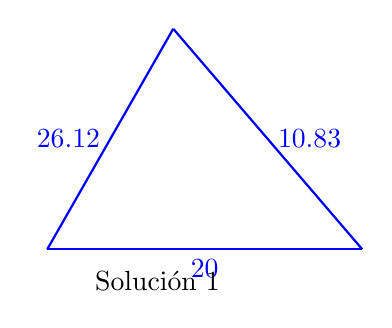
\begin{tikzpicture}[scale=0.2]
    % Triángulo 1
    \coordinate (A1) at (0,0);
    \coordinate (B1) at (20,0);
    \coordinate (C1) at (8,14);

    \draw[thick,blue] (A1) -- (B1) node[midway,below] {20};
    \draw[thick,blue] (B1) -- (C1) node[midway,right] {10.83};
    \draw[thick,blue] (C1) -- (A1) node[midway,left] {26.12};

    \node at (7,-2) {Solución 1};
\end{tikzpicture}
\hspace{2cm}
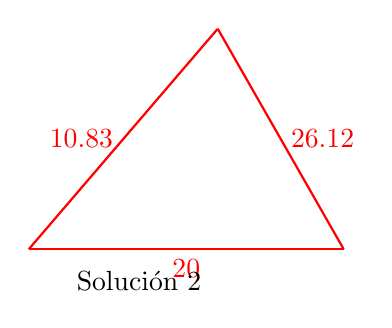
\begin{tikzpicture}[scale=0.2]
    % Triángulo 2
    \coordinate (A2) at (0,0);
    \coordinate (B2) at (20,0);
    \coordinate (C2) at (12,14);

    \draw[thick,red] (A2) -- (B2) node[midway,below] {20};
    \draw[thick,red] (B2) -- (C2) node[midway,right] {26.12};
    \draw[thick,red] (C2) -- (A2) node[midway,left] {10.83};

    \node at (7,-2) {Solución 2};
\end{tikzpicture}
\end{center}

\textbf{Respuesta:}
\[
\boxed{\begin{aligned}
\text{Hay exactamente 2 triángulos posibles} \\
\text{Ambos son acutángulos} \\
\text{Ambos tienen el mismo perímetro: } 56.95 \text{ cm} \\
\text{Lados: } (20, 26.12, 10.83) \text{ o } (20, 10.83, 26.12)
\end{aligned}}
\]

La variedad existe porque el área y un ángulo no determinan únicamente un triángulo cuando conocemos solo un lado.
\end{solucion}

\begin{solucion}[title=Solución: El Ingeniero de Estructuras]
\textbf{Análisis del equilibrio de fuerzas:}

Para el equilibrio, la suma vectorial de las fuerzas debe ser cero. Esto significa que las fuerzas forman un triángulo cerrado cuando se dibujan como vectores.

\textbf{Paso 1:} El triángulo de fuerzas.

Las fuerzas de 1000 N, 1200 N y 800 N deben formar un triángulo. Usemos la ley del coseno para encontrar los ángulos entre las fuerzas.

Para el ángulo entre las fuerzas de 1000 N y 1200 N:
\[
800^2 = 1000^2 + 1200^2 - 2(1000)(1200)\cos\alpha
\]
\[
640000 = 1000000 + 1440000 - 2400000\cos\alpha
\]
\[
\cos\alpha = \frac{2440000 - 640000}{2400000} = \frac{1800000}{2400000} = 0.75
\]
\[
\alpha = 41.41^\circ
\]

\textbf{Paso 2:} Relación con el triángulo en el suelo.

El ángulo entre las fuerzas corresponde al ángulo opuesto en el triángulo del suelo. Si el ángulo entre las fuerzas desde A y B es $41.41^\circ$, entonces el ángulo C en el triángulo ABC es $180^\circ - 41.41^\circ = 138.59^\circ$.

\textbf{Paso 3:} Calcular AC.

Usando la ley del coseno en el triángulo ABC:
\[
AC^2 = AB^2 + BC^2 - 2 \cdot AB \cdot BC \cdot \cos C
\]
\[
AC^2 = 30^2 + 40^2 - 2(30)(40)\cos 138.59^\circ
\]
\[
AC^2 = 900 + 1600 - 2400(-0.75) = 2500 + 1800 = 4300
\]
\[
AC = 65.57 \text{ m}
\]

\textbf{Paso 4:} Los otros ángulos del triángulo.

Usando la ley del seno:
\[
\frac{\sin A}{BC} = \frac{\sin C}{AC}
\]
\[
\sin A = \frac{40 \cdot \sin 138.59^\circ}{65.57} = \frac{40 \cdot 0.661}{65.57} = 0.403
\]
\[
A = 23.78^\circ
\]
\[
B = 180^\circ - 138.59^\circ - 23.78^\circ = 17.63^\circ
\]

\textbf{Paso 5:} Centro de gravedad del sistema.

El centro de gravedad está en el centroide del triángulo de fuerzas, ponderado por las magnitudes:
\[
\vec{G} = \frac{1000\vec{A} + 1200\vec{B} + 800\vec{C}}{1000 + 1200 + 800} = \frac{1000\vec{A} + 1200\vec{B} + 800\vec{C}}{3000}
\]

Si ubicamos el origen en A:
- A está en (0, 0)
- B está en (30, 0)
- C está en aproximadamente (-32.8, 56.8)

\[
G_x = \frac{1000(0) + 1200(30) + 800(-32.8)}{3000} = \frac{36000 - 26240}{3000} = 3.25 \text{ m}
\]
\[
G_y = \frac{1000(0) + 1200(0) + 800(56.8)}{3000} = \frac{45440}{3000} = 15.15 \text{ m}
\]

\begin{center}
\begin{tikzpicture}[scale=0.08]
    % Triángulo en el suelo
    \coordinate (A) at (0,0);
    \coordinate (B) at (30,0);
    \coordinate (C) at (-32.8,56.8);

    \draw[thick] (A) -- (B) node[midway,below] {30 m};
    \draw[thick] (B) -- (C) node[midway,above right] {40 m};
    \draw[thick] (C) -- (A) node[midway,left] {65.57 m};

    % Centro de gravedad
    \filldraw[red] (3.25,15.15) circle (1) node[right] {G};

    % Fuerzas (vectores)
    \draw[blue,-{Latex},very thick] (A) -- ++(10,0) node[below] {1000 N};
    \draw[blue,-{Latex},very thick] (B) -- ++(12,0) node[below] {1200 N};
    \draw[blue,-{Latex},very thick] (C) -- ++(8,0) node[below] {800 N};

    \node at (A) [below left] {A};
    \node at (B) [below right] {B};
    \node at (C) [above left] {C};
\end{tikzpicture}
\end{center}

\textbf{Reconfiguración:}

Sí es posible reconfigurar manteniendo las mismas fuerzas. Las fuerzas determinan los ángulos del triángulo pero no su tamaño. Podemos escalar el triángulo manteniendo los ángulos.

\textbf{Respuesta:}
\[
\boxed{\begin{aligned}
\text{1. Ángulo entre A y B desde la torre} &= 41.41^\circ \\
\text{2. Distancia AC} &= 65.57 \text{ m} \\
\text{3. Ángulos: } A &= 23.78^\circ, \, B = 17.63^\circ, \, C = 138.59^\circ \\
\text{4. Centro de gravedad} &= (3.25, 15.15) \text{ m desde A} \\
\text{5. Sí es posible reconfigurar} &\text{ (escalando el triángulo)}
\end{aligned}}
\]
\end{solucion}